\chapter{Critical Evaluation}
\label{chap:evaluation}

\section{Analysis of Word Lists}
\begin{figure}[ht]
\begin{subfigure}[b]{\textwidth}
\centering
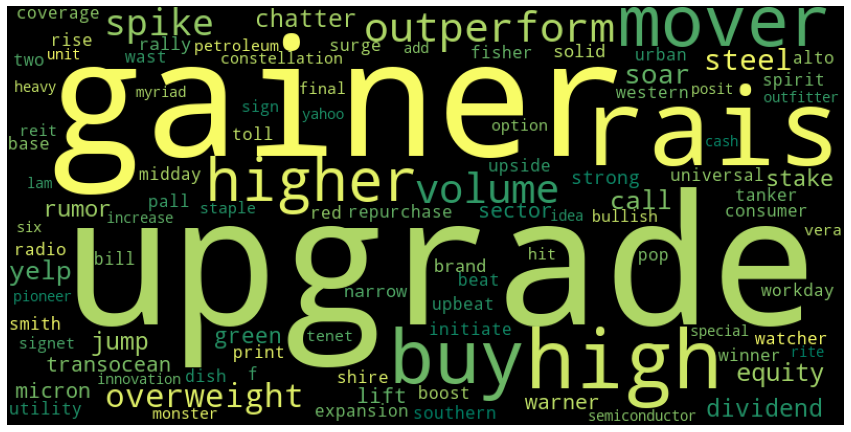
\includegraphics[scale=0.4]{pics/positive.png}
\caption{Positive words}
\end{subfigure}

\begin{subfigure}[b]{\textwidth}
\centering
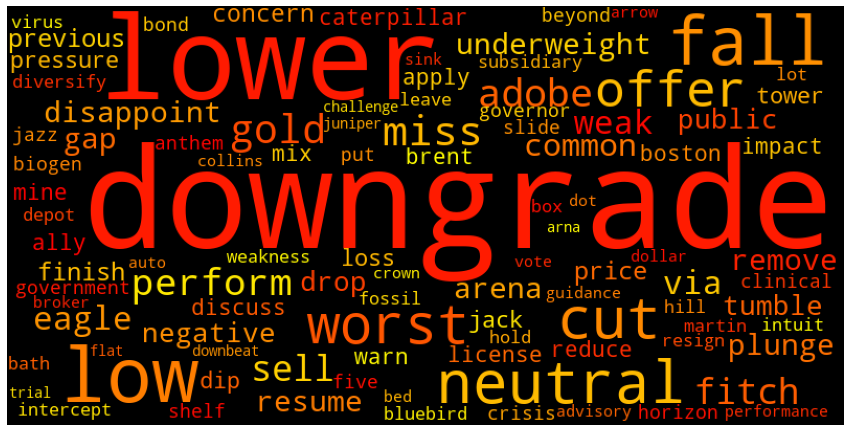
\includegraphics[scale=0.4]{pics/negative.png}
\caption{Negative words}
\end{subfigure}
\caption[Word clouds]{Word clouds demonstrating sentiment charged words. Font size corresponds to average tone across all training samples}
\label{wordclouds}
\end{figure}

Following the construction of matrix $O$, figure \ref{wordclouds} demonstrates the list of sentiment charged words on average over all training 19 windows. At each training and validation window, the sentiment lists are generated completely from scratch, and while there is some overlap, each list can vary significantly. The font size corresponds to the average tone (calculated by $\frac{1}{2}(O_+ - O_-)$) of the words across all windows. Of the top 50 positive sentiment words, the following appeared in at least 15 of the 19 windows, with words highlighted in \textbf{bold} appearing in all windows:
\begin{center}
      \textit{author, rumor, volume, repurchase, rais(e)} \textbf{gainer, mover, high, upgrade}
\end{center}

\noindent
The following words appear in at least 15 of the 19 windows with respect to top 50 negative sentiment words with words highlighted in \textbf{bold} appearing in all windows:
\begin{center}
      \textit{offer, negative, neutral, public, low} \textbf{miss, lower, loser, cut, fall, weak downgrade, underweight}
\end{center}

Simply by inspection, each group appears reasonable, in the sense that many of the words with high values in either sentiment could be assumed. However, some words are somewhat surprising and this may offer an insight into subconsious bias that exists in writing headlines as opposed to article bodies. For example, the word \textit{volume} is, under normal circumstances, a sentiment neutral word, but according to the model generated by SESTM, is a highly positive word. Examples of headlines including this word include:
\begin{itemize}
      \item \textit{Agilent spikes to high of \$60.40 on Volume}
      \item \textit{Markets gather some momentum as volume remains light, geopolitical tension improving}
      \item \textit{Tuesday's Mid-day options for volume leaders}
\end{itemize}

Observing these headlines, it is clear that the words are being used in a positive context, and this could be due to subconscious usage of the word when constructing such headlines. However, another explanation could be overfitting. Included in the sample are headlines from `Benzinga', which is a company that offers realtime news articles, and has a significant quantity of headlines of the form \textit{Benzinga's top upgrades} (around 16,000 headlines from the entire dataset) and \textit{Benzinga's volume} (with around 2,000). This could be seen as an issue of overfitting and may skew these words' sentiment value meaning that it is not reflective of the true sentiment of the word when not used in the context of Benzinga. However, both `upgrade' and `volume' appear multiple times in the word lists for bigrams \footnote{Information on bigram computation further on} with different combinations of words, meaning that there is positive sentiment attached to these words without the context of Benzinga.

When compared to the Harvard IV and Loughran McDonald dictionaries, we find that the majority of words labelled with sentiment according to our model are not in either dictionary. The negative sentiment words have much higher overlap, with 13 of the top 50 words appearing in the LM dictionary, while only 3 appear in the H4. Conversely, only 6 words overlap LM in the positive tone, while 5 words overlap the H4 dictionary. Furthermore, many words that are included in either dictionary are determined to be sentiment neutral by the model. This is because the model is trained on a sample of headlines and the vocabulary used in headlines is vastly different to that in everyday use or 10-k filings in the case of LM. Headline vocabulary often contains much more impactful words, as it is intended to be a punchy, attention grabbing piece of text. Often, words that are typically used in headlines are rarely found outside of the context of headlines \cite{language-newspapers}. For this reason, the lexicons of the model, and that of H4 and LM differ.

\subsection{Bigrams}
The order in which words appear in can have a profound effect on the sentiment of a word. This order sentiment can be captured by exploring the dictionary when constructed from \textit{bigrams} as opposed to unigrams alone. By combining both of these dictionaries, it is possible to gain a clearer understanding of the true sentiment of a headline.      

\section{Daily returns}

\begin{figure}[!ht]
      \centering
\begin{tikzpicture}
\begin{axis}[scale only axis, height=8cm, width=\textwidth*.9, grid=both,
      legend pos=north west,
      date coordinates in=x, date ZERO=2019-01-01, xticklabel=\month-\year,ymin=-50,ymax=75,
      xtick={2019-01-01,2019-02-01,2019-03-01,2019-04-01,2019-05-01,2019-06-01,2019-07-01,2019-08-01,2019-09-01,2019-10-01,2019-11-01,2019-12-01,2020-01-01,2020-02-01,2020-03-01,2020-04-01,2020-05-01,2020-06-01},
      xticklabel style={
            rotate=60,
      },
       xmin=2019-01-01,
       xmax=2020-06-08]
\addplot [red, very thick, mark=none] table [header=true,x=date,y=EW-L, col sep=comma]{data/one-day-ahead.csv};
\addplot [blue, very thick, mark=none] table [header=true,x=date,y=EW-S, col sep=comma]{data/one-day-ahead.csv};
\addplot [black, very thick, mark=none] table [header=true,x=date,y=EW-LS, col sep=comma]{data/one-day-ahead.csv};
\addplot [red, very thick, dotted, mark=none] table [header=true,x=date,y=VW-L, col sep=comma]{data/one-day-ahead.csv};
\addplot [blue, very thick, dotted, mark=none] table [header=true,x=date,y=VW-S, col sep=comma]{data/one-day-ahead.csv};
\addplot [black, very thick, dotted, mark=none] table [header=true,x=date,y=VW-LS, col sep=comma]{data/one-day-ahead.csv};
% \draw ({axis cs:2020-03-11,0}|-{rel axis cs:0,0}) -- ({axis cs:2020-03-11,0}|-{rel axis cs:0,1})
 \draw[green, very thick] (axis cs: 2020-03-11,\pgfkeysvalueof{/pgfplots/ymin}) -- 
                      (axis cs: 2020-03-11,\pgfkeysvalueof{/pgfplots/ymax})node[anchor=west,rotate=90]{Coronavirus declard pandemic};
                
\legend{L EW, S EW, LS EW, L VW, S VW, LS VW}

\end{axis}
\end{tikzpicture}
\caption[Daily cumulative log returns]{Cumulative log returns for each formation over the out of sample headlines}
\label{graph-returns}
\end{figure}

\begin{table}[!ht]
\begin{center}
\begin{tabular}{lccccccc}
      \toprule
      & Sharpe &  Average & Daily & \multicolumn{2}{c}{FF3} & \multicolumn{2}{c}{FF5} \\
      \cmidrule(lr){5-6}
      \cmidrule(lr){7-8}
      % \cmidrule(lr){9-10}
      Formation & Ratio & Return & Turnover & $\alpha$ & $R^2$ & $\alpha$ & $R^2$ \\
      \midrule
      EW LS & 0.19 & 2.61 & & 0.73 & 1.46\% & 1.23 & 1.62\% \\
      EW L & 0.7 & 10.09 & & 8.39 & 26.6\% & 8.55 & 27.32\% \\
      EW S & -0.57 & -7.47 & & -8.36 & 24.29\% & -8.02 & 24.87\% \\
      VW LS & -0.14 & -0.6 & & -2.71 & 4.45\% & -2.87 & 4.47\% \\
      VW L & -0.28 & -2.51 & & -5.29 & 22.04\% & -5.89 & 23.52\% \\
      VW S & 0.09 & 1.91 & & 1.88 & 29.57\% & 2.32 & 30.65\% \\
      \bottomrule
\end{tabular}
\caption{Performance of Daily News Sentiment Portfolios one day ahead}
\label{portfolio-performance}
\end{center}
\end{table}


Using the headlines that were saved for out of sample testing, a portfolio is constructed for each day. On average, 353 firms have articles linked to them on a given day, and of these, almost half of these headlines contain one or more sentiment words (are not marked neutral by the model). According to the constraints ($\widehat p_i < 0.5$ for a stock to be bought, and vice versa for a stock to be sold), there are some days where less than 100 stocks form the portfolio, in which case we trade with the largest value possible. On average, the long side of the portfolio has 40 stocks, while the short side has 48, therefore the average number of stocks in the portfolio is 88.

Table \ref{portfolio-performance} describes the performance of the constructed portfolios. The two investment methods (equal and value weighted) are split up into the Long-Short combined portfolio (L-S), and the long (L) and short (S) legs are also displayed separately for comparison purposes. The daily turnover section displays the average turnover each day, which would be 100\% as the profit is liquidated at the end of each day, but some stocks are retained the following day. A turnover of 90\% (as in VW L) implies that on average 1 in 10 stocks are retained the following day. This could be due to headlines or news articles that are concerning the same events (stale news), or repeat sentiment headlines as a story unfolds over a number of days.

The FF3 and FF5 sections refer to Fama French 3 and 5 factor regression respectively, while the $\alpha$ concerns the intercept. The higher percentage of the average returns that the $\alpha$ value is refers to the amount of private information held in the investment. In other words, if the $\alpha$ is a very small percentage of the generated returns, then the returns that an investment has generated can be explained by regular movement in the markets, and there is no private information that is being used to generate profit.

This figure clarifies identifies three key facts: firstly, none of these formations are profitable, with the only formation that is profitable being the equal weighted long strategy with a Sharpe ratio of 0.7, indicating that the profit versus risk ratio is beneficial. The second fact that the equal weighted formation outperforms the value weighted formation significantly in the long leg, while the short leg favours the value weighted formation. Fundamentally, this means that the trained model is better at detecting positive sentiment about smaller stocks than that of larger stocks, while also being better at detecting negative sentiment in larger stocks than smaller stocks. This is due to the nature of headlines, as, while they are intended to summarise the contents of a news article, the language used favours information that is likely to generate clicks and views. Small stocks performing well and large, supposedly stable stocks performing poorly are more likely to incentivise a user to click on the full article than their respective counterparts, meaning these are more likely to be included in the headline itself. Furthermore, the risk of the market lies with the party who shorts a stoc %todo: continue this explanation

Figure \ref{graph-returns} details the cumulative log returns over the entire out of sample dataset. Here, The performance of each of the legs are relatively steady in their respective directions until March 2020. At this point, the profits of the short legs skyrocket, while that of the long section plummet --- especially for the value weighted portfolios. This is due to the Coronavirus outbreak, as it was officially declared a pandemic on March 11 2020, indicted by the vertical green line on the graph. This, of course, caused stocks to crash worldwide, and was felt particularly by large stocks, before recovering a short while later. This also clearly highlights a limitation with all lexicon based sentiment analysis methods, whether they use supervised learning signals, or use a manually labelled dictionary: they are unable to adapt to rapid changes. Since the COVID-19 virus did not exist during the training and validation samples, the model has no information on the sentiment of headlines that would discuss this, and would ignore it. Naturally, if the model was retrained using data from this time period, it would be able to detect such headlines in the future, but the crux of the issue is that it is impossible to obtain enough information to allow the model to react to such drastic changes in the market.

%todo: describe what FF3 and 5 is and why anyone should care that I used it. Also describe basis points and how I calculated that. Also describe average turnover.

%todo: value weighted did better than equal weighted. This was different than when the findings from article bodies. This could be because headlines are more likely to give you information abuot big companies as this generates clicks...?

%todo: alphas are all very similar to daily turnover. Good because it means that this is something new I'm bringing to the table, not just old boring shit everyone knows already


\section{Speed of information Assimilation}
%TODO plot graphs of day 0 to day 7 average returns to show data assimilation

In the previous sections, we explore the relationship between the sentiment score of a headline calculated by the model and the changes in price the following day. Here, we explore the relationship between the changes in price after differing delays to investigate timing responses.

\begin{table}[!ht]
\begin{center}
\begin{tabular}{lccccccc}
      \toprule
      & Sharpe &  Average & Daily & \multicolumn{2}{c}{FF3} & \multicolumn{2}{c}{FF5} \\
      \cmidrule(lr){5-6}
      \cmidrule(lr){7-8}
      % \cmidrule(lr){9-10}
      Formation & Ratio & Return & Turnover & $\alpha$ & $R^2$ & $\alpha$ & $R^2$ \\
      \midrule
      \multicolumn{8}{c}{Day $t-1$} \\
      EW LS & 15.53 & 258.76 & & 259.78 & 4.92\% & 259.21 & 7.6\% \\
      EW L & 7.23 & 138.28 & & 140.4 & 7.78\% & 140.33 & 9.12\% \\
      EW S & 7.84 & 120.48 & & 118.68 & 29.62\% & 118.18 & 29.78\% \\
      VW LS & 12.72 & 164.11 & & 164.44 & 3.4\% & 163.49 & 6.23\% \\
      VW L & 5.26 & 76.57 & & 76.11 & 14.2\% & 76.35 & 15.76\% \\
      VW S & 6.58 & 87.55 & & 87.63 & 28.88\% & 86.44 & 29.39\% \\
      \multicolumn{8}{c}{Day $t+0$} \\
      EW LS & 10.0 & 113.75 & & 110.15 & 4.11\% & 110.42 & 4.25\% \\
      EW L & 2.5 & 34.18 & & 31.59 & 23.47\% & 32.09 & 24.37\% \\
      EW S & 4.83 & 79.57 & & 77.87 & 23.08\% & 77.64 & 23.36\% \\
      VW LS & 9.61 & 95.39 & & 93.13 & 4.79\% & 93.42 & 4.93\% \\
      VW L & 2.78 & 30.1 & & 27.12 & 30.44\% & 27.53 & 31.03\% \\
      VW S & 4.77 & 65.29 & & 65.31 & 24.58\% & 65.2 & 25.13\% \\
      \multicolumn{8}{c}{Day $t+1$} \\
      EW LS & 0.19 & 2.61 & & 0.73 & 1.46\% & 1.23 & 1.62\% \\
      EW L & 0.7 & 10.09 & & 8.39 & 26.6\% & 8.55 & 27.32\% \\
      EW S & -0.57 & -7.47 & & -8.36 & 24.29\% & -8.02 & 24.87\% \\
      VW LS & -0.14 & -0.6 & & -2.71 & 4.45\% & -2.87 & 4.47\% \\
      VW L & -0.28 & -2.51 & & -5.29 & 22.04\% & -5.89 & 23.52\% \\
      VW S & 0.09 & 1.91 & & 1.88 & 29.57\% & 2.32 & 30.65\% \\
      \bottomrule
\end{tabular}
\caption{Performance of Daily News Sentiment Portfolios day $t-1$ to day $t+1$}
\label{portfolio-performance-day-1}
\end{center}
\end{table}

Table \ref{portfolio-performance-day-1} portays the returns of different holding lengths on returns. For day $t-1$ and $t+0$, these are purely theoretical and serve only as an insight into the models performance. 

The day $t-1$ section explores portfolios created the day before a headline is released. The portfolios are constructed in the same manner as table \ref{portfolio-performance}, however, the theoretical portfolios crafted here are using headlines that have not yet been released. By doing so, we investigate how estimated sentiment score $\widehat p_i$ picks up on stale news. This is reflected in the entirely infeasible Sharpe ratios of 15.53 and 12.72 for equal and value weighted portfolio formations respectively. 

The day $t + 0$ section explores a portfolio crafted on the same day as the headline is released, providing an insight into how the estimated sentiment score picks up on fresh news. 
\begin{figure}[!ht]
      \centering
\begin{tikzpicture}
\begin{axis}[scale only axis, height=8cm, width=\textwidth*.9, grid=both,
      legend pos=north west,
      ymin=-15,ymax=20,
      xtick={1,2,3,4,5,6},
      xticklabels={Day+1, Day+2,Day+3,Day+4,Day+5,Day+6,Day+7,Day+8,Day+9,Day+10},
      xmin=1,
      xmax=6]
\addplot [black, very thick, mark=x] table [header=true,x=day,y=avg-LS, col sep=comma]{data/speed-assimilation.csv};
\addplot [red, very thick, mark=x] table [header=true,x=day,y=avg-L, col sep=comma]{data/speed-assimilation.csv};
\addplot [blue, very thick, mark=x] table [header=true,x=day,y=avg-S, col sep=comma]{data/speed-assimilation.csv};
\legend{L-S, L, S}
\end{axis}
\end{tikzpicture}
\label{speed-assimilation}
\caption[Graph of average daily returns for different holding periods]{Average daily returns for different holding periods. If article is released on day $t$, portfolio is created on day $t+(n-1)$ and sold on day $t+n$ where $n$ is the value indicated by the x axis}
\end{figure}


\section{Comparison to other methods}
%TODO create table of regression on LM and H4 dictionaries to show information not captured by each

\section{What to do}

{\bf A topic-specific chapter} 
\vspace{1cm} 

\noindent
This chapter is intended to evaluate what you did.  The content is highly 
topic-specific, but for many projects will have flavours of the following:

\begin{enumerate}
\item functional  testing, including analysis and explanation of failure 
      cases,
\item behavioural testing, often including analysis of any results that 
      draw some form of conclusion wrt. the aims and objectives,
      and
\item evaluation of options and decisions within the project, and/or a
      comparison with alternatives.
\end{enumerate}

\noindent
This chapter often acts to differentiate project quality: even if the work
completed is of a high technical quality, critical yet objective evaluation 
and comparison of the outcomes is crucial.  In essence, the reader wants to
learn something, so the worst examples amount to simple statements of fact 
(e.g., ``graph X shows the result is Y''); the best examples are analytical 
and exploratory (e.g., ``graph X shows the result is Y, which means Z; this 
contradicts [1], which may be because I use a different assumption'').  As 
such, both positive {\em and} negative outcomes are valid {\em if} presented 
in a suitable manner.

% -----------------------------------------------------------------------------
